$subject$=Физические основы компьютерных \\ и сетевых технологий
$teacher$=Лекции Герта А. В.
$date$=19.05.2025

\section{Лекция 15. Квантовое туннелирование}

В квантовой механике физические величины описываются не числами, как в классической механике, а \textbf{операторами} — специальными математическими правилами, действующими на волновые функции. Квантовые операторы — это символические обозначения преобразований, сопоставляющих одной волновой функции другую. Например, если $\Psi(x, y, z, t)$ — волновая функция частицы, то оператор $\hat{F}$ действует на неё следующим образом:
\[
\chi(x, y, z, t) = \hat{F} \Psi(x, y, z, t).
\]

Каждой классической величине $F(x, y, z, p_x, p_y, p_z)$ соответствует квантовый оператор $F(\hat{x}, \hat{y}, \hat{z}, \hat{p}_x, \hat{p}_y, \hat{p}_z)$. Например, координата и импульс в одномерном случае заменяются на:
\[
\hat{x} = x, \quad \hat{p}_x = -i\hbar \frac{\partial}{\partial x},
\]
где $\hbar$ — приведённая постоянная Планка.

Большинство операторов в квантовой механике — линейные. Это означает, что:
\[
\hat{F}(a\Psi_1 + b\Psi_2) = a\hat{F}\Psi_1 + b\hat{F}\Psi_2,
\]
для любых комплексных чисел $a$ и $b$ и функций $\Psi_1, \Psi_2$.

Особую роль играет \textbf{гамильтониан} $\mathcal{H}$ — оператор полной энергии системы. В классической механике энергия выражается через функцию Гамильтона $H(q, p)$, в квантовой механике она становится оператором $\mathcal{H}$, действующим на волновую функцию.

Если при действии оператора $\hat{F}$ на некоторую функцию $\psi(\xi)$ получается та же функция, умноженная на число $\lambda$, то $\psi$ называется \textbf{собственной функцией} оператора, а $\lambda$ — соответствующим \textbf{собственным значением}:
\[
\hat{F} \psi(\xi) = \lambda \psi(\xi).
\]
Собственные значения операторов физических величин соответствуют измеряемым значениям этих величин.

Одним из важнейших свойств квантовой механики является принцип суперпозиции: если $\Psi_1$ и $\Psi_2$ — допустимые состояния системы, то любая их линейная комбинация
\[
\Psi = C_1 \Psi_1 + C_2 \Psi_2
\]
тоже представляет возможное состояние, где $C_1, C_2 \in \mathbb{C}$. В общем случае:
\[
\Psi = \sum_{i=1}^n C_i \Psi_i.
\]

Фундаментальное уравнение квантовой механики — это \textbf{уравнение Шрёдингера}. В общем (временном) виде оно записывается так:
\[
i\hbar \frac{\partial \Psi(x, t)}{\partial t} = \hat{\mathcal{H}} \Psi(x, t),
\]
где гамильтониан $\hat{\mathcal{H}}$ для частицы массы $m$ в потенциале $U(x)$ имеет вид:
\[
\hat{\mathcal{H}} = -\frac{\hbar^2}{2m} \frac{\partial^2}{\partial x^2} + U(x).
\]
Таким образом, уравнение Шрёдингера принимает форму:
\[
i\hbar \frac{\partial \Psi(x, t)}{\partial t} = -\frac{\hbar^2}{2m} \frac{\partial^2 \Psi}{\partial x^2} + U(x)\Psi.
\]

В случае, когда потенциал не зависит от времени, можно искать \textbf{стационарные} решения в виде $\Psi(x, t) = \psi(x)e^{-iEt/\hbar}$. Тогда уравнение Шрёдингера переходит в стационарную форму:
\[
-\frac{\hbar^2}{2m} \frac{d^2 \psi}{dx^2} + U(x)\psi = E\psi,
\]
или, что то же самое:
\[
\frac{d^2 \psi}{dx^2} + \frac{2m}{\hbar^2}(E - U(x))\psi = 0.
\]

Примером задачи на стационарное уравнение Шрёдингера является движение частицы в бесконечно глубокой потенциальной яме. Пусть частица заключена между двумя бесконечными стенками на расстоянии $L$, тогда $U(x) = 0$ при $0 < x < L$ и $U(x) = \infty$ вне этого интервала. Решение принимает вид:
\[
\psi_n(x) = \sqrt{\frac{2}{L}} \sin\left( \frac{n\pi x}{L} \right), \quad n = 1, 2, 3, \ldots
\]
с дискретными значениями энергии:
\[
E_n = \frac{n^2 \pi^2 \hbar^2}{2mL^2}.
\]

\begin{wrapfigure}{R}{0pt}
    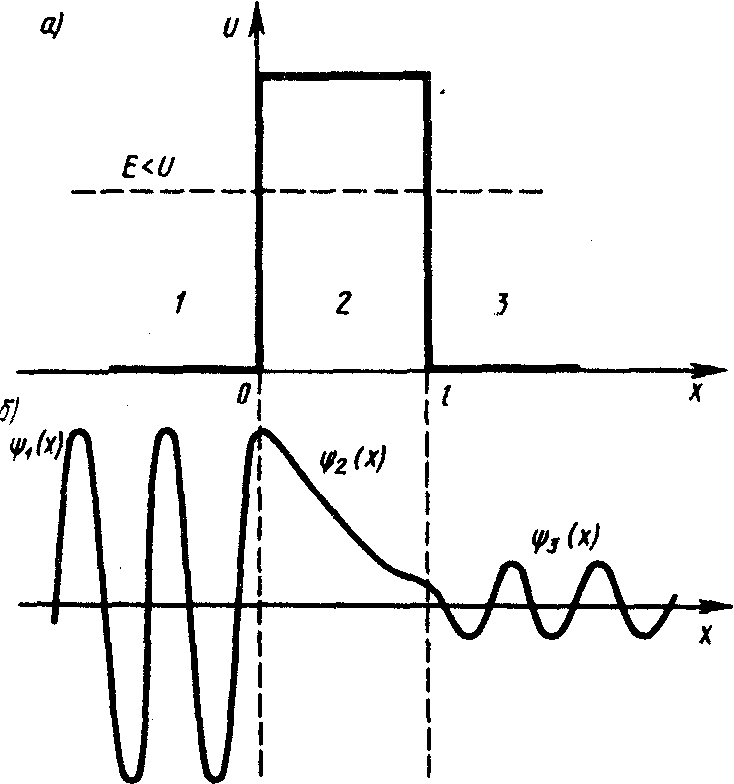
\includegraphics[width=5cm]{physics2/images/physics2_2025_05_19_1}
\end{wrapfigure}

Если потенциальный барьер конечной высоты, но выше энергии частицы, то классически она не может его преодолеть. Однако в квантовой механике волновая функция затухает, но не обнуляется в пределах барьера:
\[
\psi(x) \sim e^{-\kappa x}, \quad \kappa = \frac{\sqrt{2m(U_0 - E)}}{\hbar}.
\]
Существует ненулевая вероятность прохождения частицы через барьер — это и есть \textbf{туннельный эффект}.

Рассмотрим также важную модель — \textbf{квантовый гармонический осциллятор}, для которого потенциал имеет вид $U(x) = \frac{1}{2} m \omega^2 x^2$. Стационарное уравнение Шрёдингера принимает форму:
\[
-\frac{\hbar^2}{2m} \frac{d^2 \psi}{dx^2} + \frac{1}{2} m \omega^2 x^2 \psi = E \psi.
\]
Решения этого уравнения — функции, содержащие многочлены Эрмита и гауссовы экспоненты. Энергетические уровни дискретны:
\[
E_n = \hbar \omega \left(n + \frac{1}{2}\right), \quad n = 0, 1, 2, \ldots
\]
Это фундаментальный результат, иллюстрирующий нулевую (невыводимую) энергию даже в основном состоянии ($n = 0$), что согласуется с принципом неопределённости Гейзенберга.

Наконец, важно упомянуть \textbf{принцип Паули}, согласно которому никакие два фермиона (например, электрона) не могут находиться в одном и том же квантовом состоянии одновременно. Это объясняет электронную структуру атомов и существование периодической таблицы элементов.
